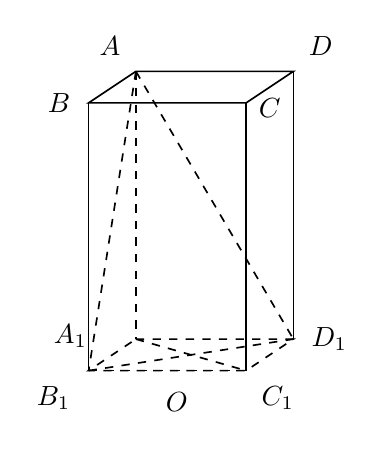
\begin{tikzpicture}[x=1cm,y=1cm,font=\normalsize,line width=.6pt]
\coordinate (A) at (0.6,4.2);
\coordinate (B) at (0,3.8);
\coordinate (C) at (2,3.8);
\coordinate (D) at (2.6,4.2);
\coordinate (Aone) at (0.6,0.8);
\coordinate (Bone) at (0,0.4);
\coordinate (Cone) at (2,0.4);
\coordinate (Done) at (2.6,0.8);
\coordinate (O) at (1.05,0.35);
% top face
\draw[solid] (A) -- (D) -- (C) -- (B) -- cycle;
% verticals
\draw[solid] (B) -- (Bone);
\draw[solid] (C) -- (Cone);
\draw[solid] (D) -- (Done);
\draw[dashed] (A) -- (Aone);
% bottom face (mostly hidden, dashed)
\draw[dashed] (Aone) -- (Done) -- (Cone) -- (Bone) -- cycle;
\draw[dashed] (Bone) -- (Done);
\draw[dashed] (Aone) -- (Cone);
% interior tetrahedron edges
\draw[dashed] (A) -- (Bone);
\draw[dashed] (A) -- (Done);
\draw[dashed] (Bone) -- (Cone);
% labels offset outward
\node[above left,xshift=-2pt,yshift=2pt] at (A) {$A$};
\node[left,xshift=-3pt] at (B) {$B$};
\node[right,xshift=1pt,yshift=-2pt] at (C) {$C$};
\node[above right,xshift=2pt,yshift=2pt] at (D) {$D$};
\node[left,xshift=-14pt,yshift=1pt] at (Aone) {$A_{1}$};
\node[below left,xshift=-3pt,yshift=-2pt] at (Bone) {$B_{1}$};
\node[below right,xshift=2pt,yshift=-2pt] at (Cone) {$C_{1}$};
\node[right,xshift=3pt] at (Done) {$D_{1}$};
\node[below,xshift=2pt,yshift=-3pt] at (O) {$O$};
\end{tikzpicture}
